\documentclass[letterpaper]{article}
\usepackage{alltt}
\usepackage{graphicx}
\usepackage{xspace}
\usepackage{color}
\usepackage{amsmath}
\definecolor{linkcolor}{RGB}{16,65,69}

\newcommand{\ttt}[1]{\texttt{#1}}
\newcommand{\projname}{\ttt{bt}\xspace}

\newenvironment{monospace}{\begin{quote}\begin{alltt}}{\end{alltt}\end{quote}}

\author{Joe Colosimo \\ \small{colosimo@mit.edu} \\ Group 6}
\date{\today}

\usepackage[colorlinks=true, linkcolor=linkcolor]{hyperref}
\title{\projname{} - A Realtime Beat Tracker \\ Microarchitecture}
\begin{document}

\maketitle

\section{Review of Overall Architecture}

    To put everything in perspective, Figure~\ref{fig:architecture} shows once
    again the overall system architecture.  This document describes the
    operation of each module in that architecture as well as their interfaces
    with one another.

    \begin{figure}
        \centering
        \includegraphics[scale=0.5]{fig/architecture.pdf}
        \caption{\projname algorithm architecture}
        \label{fig:architecture}
    \end{figure}


\section{Top Level}

    The top level module of \projname{} handles inter-module communication as
    well as sample injection and hardware output.

    \subsection{Interface to Hardware Architecture}

    The hardware produces audio samples and then requires a handshake to read
    the sample.  From the hardware side, the \ttt{sample\_injector} module
    provides the following signals:

    \begin{center}
    \begin{tabular}{|r|l|}
        \hline
        \ttt{sample} & \ttt{out std\_logic\_vector(13 downto 0)} \\ \hline
        \ttt{sample\_rdy} & \ttt{out std\_logic} \\ \hline
        \ttt{sample\_rd} & \ttt{in std\_logic} \\ \hline
    \end{tabular}
    \end{center}

    \projname{} therefore waits for input \ttt{sample\_rdy} to go high, at
    which point it captures \ttt{sample} and asserts \ttt{sample\_rd = '1'} for
    one clock cycle.  It enqueues the sample to the beat classifier's input
    FIFO through its \ttt{InjectSample} method.

    \subsection{Output}
        
    The output of the top module is a (wide) parallel bus that is an array of
    the attempted tempos and their respective likelihoods.  The hardware
    architecture takes care of splitting this bus up into bytes for output via
    serial.

    \subsection{Submodules}

    There is a single beat classifier, a vector of metronomes, and a single
    metronome bank controller.  As discussed later, the top level takes care of
    tasks such as iterating a command, such as \ttt{SetMetronomeTempo} from the
    metronome bank controller to all of the metronomes.


\section{Beat Classifier}

    The beat classifier handles the process of receiving injected audio samples
    and determining when the audio stream has likely produced a beat.


    \subsection{Operation}
        
    The beat classification algorithm essentially compares the local energy of
    a small sample window to the average energy of a much larger window.  If
    there is significant deviation of the local energy from the average energy
    (either positive or negative), then the beat classifier reports that it saw
    a beat.

    It runs a round of this every time it receives a sample via its
    \ttt{InjectSample} method, described below.  When a new sample has been
    presented, it computes this instantaneous energy of the sample, by squaring
    it and accumulates this to the \ttt{LocalEnergy} register.  When $N_L$ of
    such samples are accumulated, we are ready to compare the local energy with
    the average energy, which is held in the \ttt{AverageEnergy} register.  If
    the local energy is different from the average energy by a factor $F$, we
    report a beat by setting a \ttt{Maybe} register valid as described in
    Section~\ref{sec:bc:metif}.

    We then update the average energy register using a simple EWMA scheme:
    \begin{equation}
        \textrm{\ttt{AverageEnergy}} = \alpha \textrm{\ttt{AverageEnergy}} +
                        (1-\alpha) \textrm{\ttt{LocalEnergy}}
    \end{equation}

    where $\alpha$ is some number less than 1 and represents the degree of
    decay.  Another way to handle the \ttt{AverageEnergy} would be to instead
    keep a buffer of local energies and take an arithmetic average.  This also
    allows us to compute the variance of the local energies, which would allow
    us to approximate $F$ far better than if it were constant.

    
    \subsection{Tunable Parameters}

    There are a few parameters here that can be fine-tuned.

    $N_L$ basically asks "how many samples corresponds to local energy?".  If
    it's too small, we may not get a good enough estimate of the signal energy
    at any given point, but if it's too large, then we could be including a
    beat with non-beat portion of the spectrum.  Experiments suggest that $N_L
    \approx 1000$ works well.

    $F$ determines just how different the local energy has to be from the
    average energy for a beat to be considered.  In practice, if we were to
    think of the ratio of local energy to average energy, $F$ usually works
    well at about 1.2 or 1.3.  However, this can vary by genre.  This is why I
    would eventually like to be able to compute the variance of local energies
    to determine a best fit for F.

    $\alpha$ determines the decay rate of the average energy.  A low value of
    $\alpha$ indicates that we want to consider recent energies much, much more
    than older energies.  However, in this case, $\alpha$ should be fairly
    high, around 0.6 or 0.7.  If $\alpha$ is too high, however, we could run
    into issues where the overall energy of the track has changed but the
    average energy doesn't quite catch up to reflect that.  $\alpha$ will be
    represented as a \ttt{FixedPoint} fraction.


    \subsection{Interface to Top-Level Injector: \ttt{InjectSample}}

    The module has a very small FIFO through which input samples come in on.
    The method \ttt{InjectSample} simply enqueues a sample for processing.
        

    \subsection{Interface to the Metronomes: \ttt{SawBeat}}
    \label{sec:bc:metif}

    For a given input sample, if the beat classifier has detected a beat,
    it delivers a message to all of the metronomes.  To do this, it
    maintains a register of type \ttt{Maybe\#(BeatLikelihood)} that it
    updates on each clock cycle where a valid value indicates that a beat
    was discovered.  The \ttt{BeatLikelihood} type is a way for the
    classifier to indicate to the metronomes just how likely it thought
    what it just saw was a beat.  This allows the metronomes to adjust
    their phase accordingly, as is discussed later in this document.

    To read this register, the beat classifier module provides a method
    called \ttt{SawBeat} that returns its contents.  The top level module
    calls this method on every clock cycle and when the value returned is
    valid, calls the \ttt{InjectBeat} method of each metronome with the
    likelihood as an argument.


\section{Metronome}

    The metronome keeps time to a given tempo.  Essentially, it's a fancy
    counter that's not unlike something that one would use as the phase ramp
    input to a lookup table for a DDS.

    \subsection{Operation}

    The metronome uses a fixed point representation where the integer part is
    only 2 bits and the decimal part is much larger (as large as possible while
    still fitting within the resource constraints).  The integer part
    represents sixteenth notes.  When it rolls over from 3 to 0, a quarter note
    has occurred.


    \subsection{Setting the Tempo: \ttt{SetTempo}}

    This sets the amount that the counter is incremented by with each clock
    cycle.  In the language of DDSes, this is the slope of the phase ramp.


    \subsection{Starting the Metronome: \ttt{Start}}

    This method resets all of the counters to 0 and enables counting.


    \subsection{Injecting a Beat: \ttt{InjectBeat}}
    
    When the beat classifier detects a beat, it indicates this to all of the
    metronomes.  The metronome responds by adjusting its counter's phase to be
    closest to the nearest sixteenth note according to the \ttt{BeatLikelihood}
    value.  It also returns the phase offset that it had to apply to achieve
    this back to the top level module (which goes on to deliver this
    information to the metronome bank controller).

    The base implementation will simply just set the phase to the nearest
    sixteenth note, but the more advanced implementation will do so linearly
    according to the \ttt{BeatLikelihood} value.  So, for example, if the value
    was 0.5, the phase will be set to halfway between its current value and the
    nearest sixteenth note.


\section{Metronome Bank Controller}

    The metronome bank controller collects all of the metronome phase
    differences and uses that to generate the parallel output stream, but also
    to set the tempos of the individual metronomes.

    For each metronome, it keeps track of an EWMA'd running average for the
    phase error.  Each time the metronome reports a phase error, the controller
    computes the new average phase error as $\alpha \textrm{\ttt{AvgPhaseErr}}
    + (1-\alpha) \textrm{\ttt{PhaseError}}$.  In this case $\alpha=0.5$.

    The parallel output stream is simply generated by shoving all the metronome
    tempos and their respective average phase errors (with 16 bits of precision)
    into a parallel bus.

    The other major thing that the controller does is with each update of the
    average phase error, is to compute their gradient.  If the maximum and
    minimum differ by a large enough factor, the bank controller will ``zoom
    in" to a new set of tempos based on where the phase error is minimal.
    Experimentation showed that it works best to close in on the convergence by
    a factor of two.  That is, if the previous range spanned 100~BPM, the next
    range should span 50~BPM, etc.



\end{document}
